\preClass{Coordinate Systems}


\videoLink{Section 1.6 Day 1}{https://www.youtube.com/playlist?list=PLYHZK3b8UFw3srUWdN3pnV1WRNsEcqx-T}


\begin{enumerate}

\item  For this problem, let $f(x)=|x|$.

\begin{enumerate}
\item Graph $f(x)=|x|$.  Then determine the domain and range of $f(x)$.\\
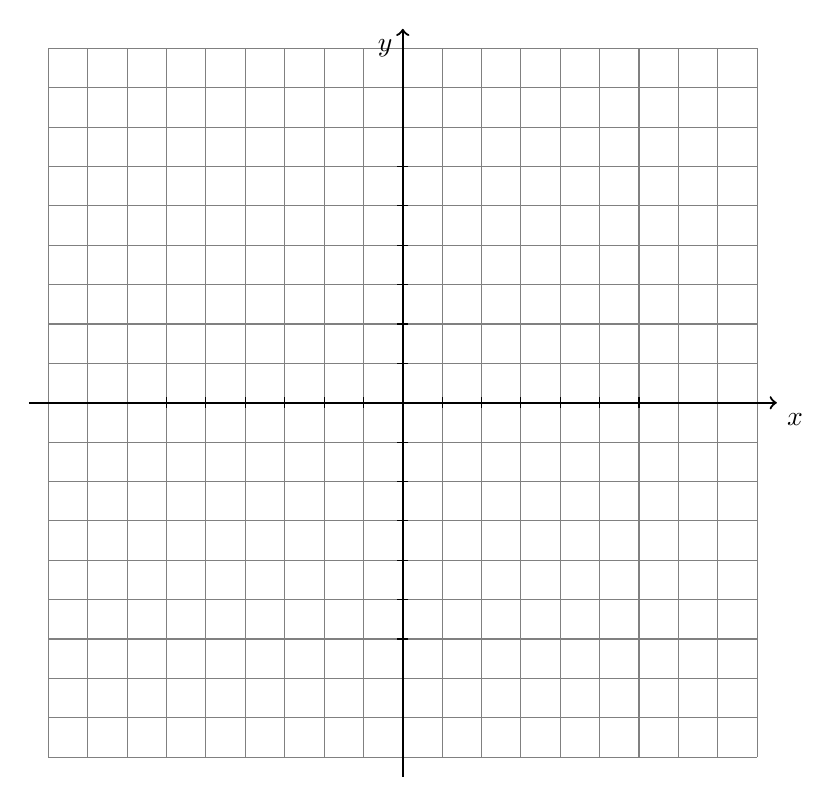
\begin{tikzpicture}[y=.5cm, x=0.5cm,font=\sffamily]
    %% ticks
    \draw[step = 1, gray] (-9,-9) grid (9,9);
    %% axis
    \draw[thick,->] (-9.5,0) -- coordinate (x axis mid) (9.5,0) node[anchor = north west] {$x$};
    \draw[thick,->] (0,-9.5) -- coordinate (y axis mid) (0,9.5) node[anchor = north east] {$y$};
    \foreach \y in {-6,-5,...,-1,1,2,...,6} {
      \draw (2pt, \y) -- (-2pt, \y);
    }
    \foreach \x in {-6,-5,...,-1,1,2,...,6} {
      \draw (\x,2pt) -- (\x,-2pt);
    }

  \end{tikzpicture}

\vfill



\item Graph and label $f(x+2)$ on the coordinate system above.  Then determine the domain and range of $f(x+2)$.

\end{enumerate}
\vfill

\newpage

\item For this problem, let $f(x)=\sqrt{x}$.
\begin{enumerate}
\item Graph $f(x)=\sqrt{x}$.  Then determine the domain and range of $f(x)$.\\
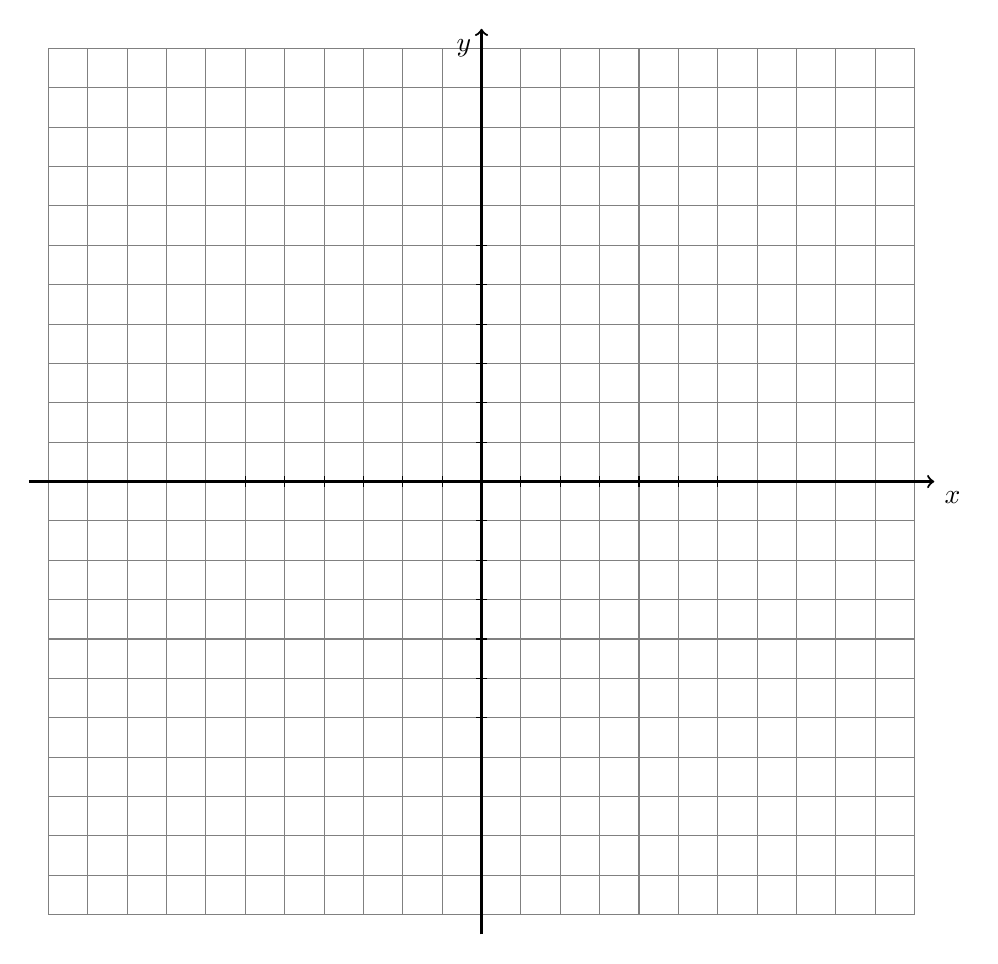
\begin{tikzpicture}[y=.5cm, x=0.5cm,font=\sffamily]
    %% ticks
    \draw[step = 1, gray] (-11,-11) grid (11,11);
    %% axis
    \draw[thick,->] (-11.5,0) -- coordinate (x axis mid) (11.5,0) node[anchor = north west] {$x$};
    \draw[thick,->] (0,-11.5) -- coordinate (y axis mid) (0,11.5) node[anchor = north east] {$y$};
    \foreach \y in {-6,-5,...,-1,1,2,...,6} {
      \draw (2pt, \y) -- (-2pt, \y);
    }
    \foreach \x in {-6,-5,...,-1,1,2,...,6} {
      \draw (\x,2pt) -- (\x,-2pt);
    }

  \end{tikzpicture}

\vfill
\item Graph and label $f(x)-3$ on the coordinate system above.  Then determine the domain and range of $f(x)-3$.\vfill
\vfill
\end{enumerate}






\end{enumerate}


